\documentclass[twoside,11pt]{homework}

\usepackage{dsfont}
\usepackage{amsmath}
\usepackage{graphicx}
\usepackage{float}

\coursename{COMS 4771 Machine Learning (Spring 2020)} 

\studname{Angela Wang}     
\studmail{aw3062@columbia.edu}
\collab{Jane Pan, Stan Liao}
\hwNo{1}      
\date{02/21/2020}  
\begin{document}
\maketitle

\section*{Problem 1} 
\subsection*{(i)}
	The likelihood function of $\theta$ is 
	\begin{align*}
		\mathcal{L}(\theta|X):=& \mathbb{P}(X|\theta) \\
		=& \prod_{i=1}^n \mathbb{P}(x_i | \theta) \tag{i.i.d.}
	\end{align*}
	where $\mathbb{P}(x_i | \theta) = \frac{1}{b-a}$ if $x\in [a,b]$, and $\mathbb{P}(x_i | \theta) = 0$ otherwise. 
	The maximum likelihood estimate is the $\theta$ that maximizes $\mathcal{L}(\theta|X)$, given by
	\begin{align*}
		 \text{arg}\max_\theta \mathcal{L}(\theta|X) 
		=  \text{arg}\max_\theta \log \mathcal{L}(\theta|X) 
		= \text{arg}\max_\theta \log \prod_{i=1}^n \mathbb{P}(x_i | \theta)
	\end{align*}
	To maximize the likelihood, we choose $a\leq \min(x_1,\dots,x_n)$, and  $b\geq \max(x_1,\dots,x_n)$,
	\begin{align*}
		& \text{arg}\max_\theta \mathcal{L}(\theta|X) \\
		= & \text{arg}\max_\theta \log \left(\frac{1}{b-a}\right)^n \\
		= & \text{arg} \max_\theta \, n \log\left(\frac{1}{b-a}\right)
	\end{align*}
	To maximize the logarithm, we should minimize $b-a$. Hence $\theta_{\text{ML}} = (a_{\text{ML}} ,b_{\text{ML}} )$, where
	\begin{align*}
		a_{\text{ML}}  &= \min(x_1,\dots,x_n) \\
		b_{\text{ML}}  &= \max(x_1,\dots,x_n)
	\end{align*}
\subsection*{(ii)}
	\begin{proof}
		Define $\eta = g(\theta)$. Suppose $g$ is bijective, then $\exists g^{-1}$ such that 
		\begin{align*}
			\mathcal{L}(\theta|X) = \mathcal{L}( g^{-1}(\eta) |X)
		\end{align*}
		whose maximum value is $\mathcal{L}(\theta_{\text{ML}}|X) $. 
		To maximize $\mathcal{L}( g^{-1}(\eta) |X)$, choose $\eta_{\text{ML}}$
		such that $g^{-1}(\eta_{\text{ML}})=\theta_{\text{ML}}$. We have $\eta_{\text{ML}}=g(\theta_{\text{ML}})$ \\ \\
		For the case when $g$ is not bijective: we can define $L(t) = max_{\theta \in g^{-1}(t)} \mathcal{L}(\theta | x)$ where we define
		$g^{-1}$ denotes the preimage rather than the inverse. $\{g^{-1}(t)\}$ denotes the set of all values $\theta$ s.t. $g(\theta) =t$ \\ \\
		If $\Omega$ is the parameter space, the MLE of $g(\theta)$ is the value $t \in g(\Omega)$ such that $L(t)$ is maximized. As noted in the conditions, $\theta _{ML} $ exists such that $\mathcal{L}(\theta| x)$ is maximized for $\theta = \theta_{ML}$. The highest possible value for $\mathcal{L}(\theta | x)$ equals the highest possible value for $max_{\theta \in g^{-1}(g(\Omega))} \mathcal{L}(\theta | x)$\\ \\
Thus, $L(t)$ across all $t \in g(\Omega) $ is maximized for $\theta_{ML} \in \{g^{-1}(t)\}$ or $g(\theta_{ML}) = t$ 
	\end{proof}
\subsection*{(iii)}
	Let $X_1,\dots, X_n \sim \mathcal{N}(\mu, \sigma^2)$ be i.i.d random variables.
\subsubsection*{(a)}
	\begin{claim}
		$\frac{1}{n} \sum_{i=1}^n X_i $ is a consistent and unbiased estimator for $\mu$.
	\end{claim}
	\begin{proof}
		By Law of Large Numbers, 
		$ \lim\limits_{n\rightarrow \infty} \frac{1}{n} \sum_{i=1}^n X_i = \mu$.\\
		Since $\mathbb{E}[\frac{1}{n} \sum_{i=1}^n X_i]
		=\frac{1}{n} \sum_{i=1}^n \mathbb{E}[X_i]
		=\frac{1}{n} \sum_{i=1}^n \mu
		=\mu
		$, the estimator is unbiased.
	\end{proof}
	\begin{claim}
		$\frac{1}{n} \sum_{i=1}^n X_i + \frac{1}{n} X_1- \frac{1}{n} X_2$ is a consistent and unbiased estimator for $\mu$.
	\end{claim}
	\begin{proof}
		By Law of Large Numbers, 
		$ \lim\limits_{n\rightarrow \infty} \frac{1}{n} \sum_{i=1}^n X_i + \frac{1}{n} X_1- \frac{1}{n} X_2 = \mu$.\\
		Since $\mathbb{E}[\frac{1}{n} \sum_{i=1}^n X_i  + \frac{1}{n} X_1- \frac{1}{n} X_2]
		=\frac{1}{n} (\sum_{i=1}^n \mathbb{E}[X_i] +  \sum_{i=1}^n \mathbb{E}[\frac{1}{n} X_1 - \frac{1}{n} X_2]
		=\frac{1}{n} (\sum_{i=1}^n \mu + \frac{\mu}{n} - \frac{\mu}{n})
		=\mu
		$, the estimator is unbiased.
	\end{proof}

\subsubsection*{(b)}	
	\begin{claim}
		$ \frac{1}{n} \sum_{i=1}^n X_i +\frac{1}{n}$ is a biased but consistent estimator for $\mu$.
	\end{claim}
	\begin{proof}
		$ \lim\limits_{n\rightarrow \infty} (\frac{1}{n} \sum_{i=1}^n X_i +\frac{1}{n})= \mu$.
		$\mathbb{E}[\frac{1}{n} \sum_{i=1}^n X_i +\frac{1}{n}]
		=\frac{1}{n} \sum_{i=1}^n \mathbb{E}[X_i] +\frac{1}{n}
		=\mu+\frac{1}{n}.
		$
	\end{proof}
	\begin{claim}
		$ \frac{1}{n} \sum_{i=1}^n X_i +\frac{1}{n^2}$ is a biased but consistent estimator for $\mu$.
	\end{claim}
	\begin{proof}
		$ \lim\limits_{n\rightarrow \infty} (\frac{1}{n} \sum_{i=1}^n X_i +\frac{1}{n^2	})= \mu$.
		$\mathbb{E}[\frac{1}{n} \sum_{i=1}^n X_i +\frac{1}{n^2}]
		=\frac{1}{n} \sum_{i=1}^n \mathbb{E}[X_i] +\frac{1}{n^2}
		=\mu+\frac{1}{n^2}.
		$
	\end{proof}
\subsubsection*{(c)}
	\begin{claim}
		$X_1$ is an unbiased but inconsistent estimator for $\mu$.
	\end{claim}
	\begin{proof}
		$X_1$ is not consistent since its distribution does not become more concentrated around $\mu$ 
		as the sample size increases.
		$\mathbb{E}[X_1] =\mu$ so $X_1$ is an unbiased estimator.
	\end{proof}
	\begin{claim}
		$X_2$ is an unbiased but inconsistent estimator for $\mu$.
	\end{claim}
	\begin{proof}
		$X_2$ is not consistent since its distribution does not become more concentrated around $\mu$ 
		as the sample size increases.
		$\mathbb{E}[X_2] =\mu$ so $X_2$ is an unbiased estimator.
	\end{proof}
\subsubsection*{(d)}
	\begin{claim}
		The constant $1$ is a biased and inconsistent estimator for $\mu$.
	\end{claim}
	\begin{proof}
		1 is not consistent since its distribution does not become more concentrated around $\mu$ 
		as the sample size increases.
		$\mathbb{E}[1] = 1 $ which doesn't necessarily equal $\mu$ so 1 is a biased estimator
	\end{proof}
	\begin{claim}
		$1+X_1$ is a biased and inconsistent estimator for $\mu$.
	\end{claim}
	\begin{proof}
		$1 + X_1$ is not consistent since its distribution does not become more concentrated around $\mu$ 
		as the sample size increases.
		$\mathbb{E}[1+X_1] = 1 + \mu \neq \mu $  so $1 + X_1$ is a biased estimator
	\end{proof}
	
\section*{Problem 2} 
\subsection*{(i)}
	Let $\Pi$ be the profit. We can write
	\begin{align*}
		\Pi &= \mathds{1}_{D\geq Q} (P-C)Q + \mathds{1}_{D\leq Q} \left[(P-C)D-C(Q-D)\right] \\
		&= -CQ +\mathds{1}_{D\geq Q} PQ+\mathds{1}_{D\leq Q} PD
	\end{align*}
	The expected profit is given by
	\begin{align*}
		\mathbb{E} [\Pi] &= -CQ+\int_Q^\infty PQ\mathbb{P}(D)dD
		+ \int_{-\infty}^Q PD\mathbb{P}(D)dD \\
		&= -CQ+ PQ\int_Q^\infty \mathbb{P}(D)dD
		+ P\int_{-\infty}^Q D\mathbb{P}(D)dD
	\end{align*}
\subsection*{(ii)}
	\begin{proof}
	Taking the derivative,
	\begin{align*}
		\frac{d\mathbb{E} [\Pi]}{dQ} &= -C + P\int_Q^\infty \mathbb{P}(D)dD
		+ PQ \frac{d}{dQ} \int_Q^\infty \mathbb{P}(D)dD
		+ P \frac{d}{dQ}  \int_{-\infty}^Q D\mathbb{P}(D)dD \\
		&= -C + P\int_Q^\infty \mathbb{P}(D)dD
		- PQ \mathbb{P}(Q)
		+ P Q\mathbb{P}(Q) \tag{Fundamental Theorem of Calculus}\\
		&=-C+P\int_Q^\infty \mathbb{P}(D)dD\\
		&=-C +P(1-F(Q))
	\end{align*}
	To maximize profit, we let $\frac{d\mathbb{E} [\Pi]}{dQ} =-C +P(1-F(Q^*)= 0$. Rearranging, we have
	\begin{align*}
		Q^*= F^{-1}\left(1-\frac{C}{P}\right)
	\end{align*}
	\end{proof}

\section*{Problem 3} 
\subsection*{(i)}
	The error rate is the probability of getting false positive or false negatives:
	\begin{align*}
		& \mathbb{P}[f_t(x)\neq y] \\
		=& \mathbb{P}[Y=y_1 | X\leq t] + \mathbb{P}[Y=y_2 | X\geq t] \\
		=& \int_{-\infty}^t  \mathbb{P}[Y=y_1 | X=x] dx + \int_{t}^\infty  \mathbb{P}[Y=y_2 | X=x] dx
	\end{align*}
\subsection*{(ii)}
	Differentiating the error rate, we have
	\begin{align*}
		& \frac{d}{dt} \mathbb{P}[f_t(x)\neq y]  \\
		=& \, \frac{d}{dt}\int_{-\infty}^t  \mathbb{P}[Y=y_1 | X=x] dx - \frac{d}{dt} \int_{\infty}^t  \mathbb{P}[Y=y_2 | X=x] dx \\
		=&\,  \mathbb{P}[Y=y_1 | X=t] - \mathbb{P}[Y=y_2 | X=t] \tag{Foundamental Theorem of Calculus}
	\end{align*}
	To minimize the error rate, we set $\frac{d}{dt} \mathbb{P}[f_t(x)\neq y] = 0$,
	\begin{align*}
		\mathbb{P}[Y=y_1 | X=t] &= \mathbb{P}[Y=y_2 | X=t] \\
		\mathbb{P}[ X=t | Y=y_1 ] \frac{ \mathbb{P}[ Y=y_1 ]}{ \mathbb{P}[ X=t]}
		&= \mathbb{P}[ X=t | Y=y_2 ] \frac{ \mathbb{P}[ Y=y_2 ]}{ \mathbb{P}[ X=t]} \tag{Bayes Rule}\\
		\mathbb{P}[ X=t | Y=y_1 ] \mathbb{P}[ Y=y_1 ] 
		&= \mathbb{P}[ X=t | Y=y_2 ] \mathbb{P}[ Y=y_2 ]
	\end{align*}
\subsection*{(iii)}
	Let the distribution of $\mathbb{P}[X|Y=y_1]$ be $\mathcal{N}(\mu_1,\sigma_1^2)$, 
	and the distribution of $\mathbb{P}[X|Y=y_2]$ be $\mathcal{N}(\mu_2,\sigma_2^2)$.
	By Bayesian Decision Theory, the Bayes error is the overlapped area under $\mathcal{N}(\mu_1,\sigma_1^2)$
	and $\mathcal{N}(\mu_2,\sigma_2^2)$. \\
	Example in which $f_t$ achieves Bayesian error rate:
	\begin{align*}
		\mathbb{P}[X|Y=y_1] &\sim \mathcal{N}(-1, 1)\\
		\mathbb{P}[X|Y=y_2] &\sim \mathcal{N}(1, 1) \\
		t&=0
	\end{align*}
	Example in which $\forall t\in \mathbb{R}$, $f_t$ does not achieve Bayesian error rate:
	\begin{align*}
		\mathbb{P}[X|Y=y_1] &\sim \mathcal{N}(0, 1)\\
		\mathbb{P}[X|Y=y_2] &\sim \mathcal{N}(0, 2) \\
	\end{align*}


\section*{Problem 4} 
\subsection*{(i)}
	\begin{proof}
		Since $M^{T} = (A^{T}A)^{T} = A^{T}A = M$, M is symmetric. 
		For any column vector $z\in \mathbb{R}^d$, $z^TMz = z^TA^TAz = (Az)^T (Az) = (Az)\cdot(Az) \geq 0$, 
		so M is positive semi-definite.
	\end{proof}
\subsection*{(ii)}
	\begin{proof}
		Base case: if $N=1$, then by definition, 
		\begin{align*}
			\beta^{(1)} &= \beta^{(0)}+ \eta  A^{T} (b-A \beta^{(0)}) \\
			&= \eta v - \eta M \beta^{(0)} \\
			&= \eta v 
		\end{align*}
		Assuming the statement $\beta^{(N)} = \eta \sum_{k=0}^{N-1} (I-\eta M)^k v$ is true for $N=n$, then for $N=n+1$ we have
		\begin{align*}
			\beta^{(n+1)} &= (I-\eta M) \beta^{(n)} + \eta v \tag{definition} \\
			&= (I-\eta M) \eta  \sum_{k=0}^{n-1} (I-\eta M)^k v + \eta v \tag{induction hypothesis} \\
			&= \eta  \sum_{k=0}^{n-1} (I-\eta M)^{(k+1)} v + \eta (I-\eta M)^0 v \\
			&= \eta  \sum_{k=1}^{n} (I-\eta M)^{(k)} v + \eta (I-\eta M)^0 v \\
			&= \eta  \sum_{k=0}^{n} (I-\eta M)^{(k)} v
		\end{align*}
	\end{proof}
\subsection*{(iii)}
	Since $M$ is a real symmetric matrix, it has a decomposition $M = P D P^{-1}$, 
	where $P$ is a matrix composed of orthogonal eigenvectors corresponding to distinct eigenvalues,
	and $D:= \text{diag}(\lambda_1,\dots, \lambda_d)$.
	\begin{align*}
		&\eta \sum_{k=0}^{N-1} (I-\eta M)^k \\
		=&\eta \sum_{k=0}^{N-1} \left(P(\text{diag} \left( 1- \eta \lambda_1, \dots, 1- \eta \lambda_d
		\right) \right)P^{-1})^k \tag{$I-\eta M$ is symmetric} \\
		=&\eta \sum_{k=0}^{N-1} P \,
		\text{diag} \left( (1- \eta \lambda_1)^k, \dots, (1- \eta \lambda_d)^k \right) P^{-1} \\
		=& P \, \text{diag} \left( \sum_{k=0}^{N-1} \eta(1- \eta \lambda_1)^k, 
		\dots, \sum_{k=0}^{N-1} \eta(1- \eta \lambda_d)^k \right) P^{-1}
	\end{align*}
	Since $I$, $M$ are symmetric, $\eta \sum_{k=0}^{N-1} (I-\eta M)^k$ is symmetric, 
	and its eiganvalues $\lambda_1',\dots, \lambda_d'$ are given by
	\begin{align*}
		\lambda_i' = \sum_{k=0}^{N-1} \eta(1- \eta \lambda_i)^k
	\end{align*}
	for any $i=1,\dots,d$.
\subsection*{(iv)}
	\begin{proof}
	We start by deriving a iterative formula for the difference
	\begin{align*}
		& ||\beta^{(N)} - \hat{\beta}||_2^2 \\
		=& \left( (I-\eta M)^N \hat\beta \right)^T \left( (I-\eta M)^N \hat\beta \right) \\
		=& \, \hat\beta^T (I-\eta M)^{2N} \hat\beta \\
		\leq& \, \hat\beta^T (I-2N\eta M) \hat\beta \tag{Taylor's Theorem} \\
		\leq& \, || I-2N\eta M ||_2 \cdot ||\hat{\beta}||_2^2 \\
		\leq & \, (1-2N\eta \lambda_{\text{min}}) ||\hat{\beta}||_2^2 
		\tag{Since $\sigma_{\text{max}}(I-2N\eta M) = 1-2N\eta \sigma_{\text{min}}(M)$} \\
		\leq& \, e^{-2N\eta\lambda_{\text{min}}}||\hat{\beta}||_2^2 
	\end{align*}
	\end{proof}




\section*{Problem 5}
\subsection*{(i)}
	There may be correlated attributes (e.g. neighborhood) that are proxies of the sensitive attribute (e.g. race). 
	Simply removing race does not decrease bias, since neighborhood still acts as a trait in classification of the data. 
	The model therefore fails to maintain fairness across the sensitive attribute.
\subsection*{(ii)}  
	\begin{proof}
	Assuming for any $a\in A$, $\mathbb{P}[\hat{Y}=1]=\mathbb{P}_a[\hat{Y}=1]$, we can write trivially
	\begin{align*}
		\mathbb{P}_0[\hat{Y}=1]&=\mathbb{P}_1[\hat{Y}=1]
	\end{align*}
	Conversely, if $\mathbb{P}_0[\hat{Y}=1]=\mathbb{P}_1[\hat{Y}=1]=:\mathbb{P}_a[\hat{Y}=1]$, then 
	\begin{align*}
		\mathbb{P}[\hat{Y}=1] &= \mathbb{P}[\hat{Y}=1|a=0]\mathbb{P}[a=0]+\mathbb{P}[\hat{Y}=1|a=1]\mathbb{P}[a=1]\\
		&= \mathbb{P}_a[\hat{Y}=1] (\mathbb{P}[a=0]+\mathbb{P}[a=1])\\
		&= \mathbb{P}_a[\hat{Y}=1]
	\end{align*}
	\end{proof}
\subsection*{(iii)}  
	\begin{claim}
		$\forall a_1, a_2  \in A\subset \mathbb{N}$, $\forall y\in \mathbb{R}$, we have 
		$$\mathbb{P}_{a_1}[\hat{Y}=y] = \mathbb{P}_{a_2}[\hat{Y}=y] 
		\Longleftrightarrow \mathbb{P}[\hat{Y}=y] = \mathbb{P}_a[\hat{Y}=y] \qquad \forall a\in A$$
	\end{claim}
	\begin{proof}
		The backward direction is trivial. For the forward direction, we write
		\begin{align*}
			 \mathbb{P}[\hat{Y}=y] &= \sum_{a_i \in A} \mathbb{P}_{a_i}[\hat{Y}=y]\mathbb{P}[a=a_i] \\
 			 &=  \mathbb{P}_a[\hat{Y}=y] \left( \sum_{a_i\in A} \mathbb{P}[a=a_i] \right) \\
			 &=  \mathbb{P}_a[\hat{Y}=y] 
		\end{align*}
	\end{proof}
	
\subsection*{(iv)}  
	We choose $k=148$ for KNN, because it gives relatively high accuracy with the same distance metric ($L_2$).
	\begin{figure}[H]
		\centering
		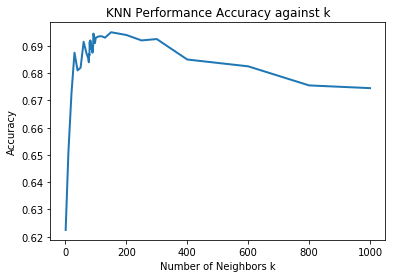
\includegraphics[scale=.5]{q5_fig/performance_vs_k.png}	
		\caption{Prediction Accuracy against k for Nearest Neighbor Algorithm}
	\end{figure}
	We use $L_2$ as the distance metric for KNN, because it gives high accuracy under $k=148$. 
	It makes sense that as $p$ approaches infinity, accuracy of KNN decreases, 
	because the distance metric becomes Chebyshev, and only the maximum difference between traits will affect the classification result.
	In this example, age will become the most influential factor.
	\begin{figure}[H]
		\centering
		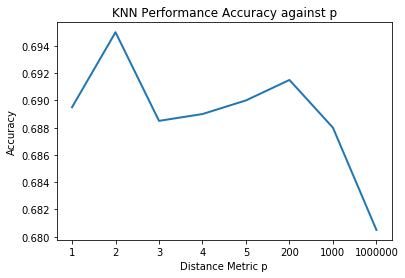
\includegraphics[scale=.5]{q5_fig/performance_vs_p.png}	
		\caption{Prediction Accuracy against k for Nearest Neighbor Algorithm}
	\end{figure}
	Table 1 summarizes the performance rate for the classifiers.
	\begin{table}[H]
	\centering
	\caption{Performance of Classifiers}
	\begin{tabular}{lr}
		Classifier   & Accuracy \\
		\textbf{MLE}   & 0.6415    \\
		\textbf{KNN}   & 0.6895        \\
		\textbf{Bayes} & 0.68
	\end{tabular}
	\end{table}
	
	
\subsection*{(v)}  
	Based on the learning curve of classifiers, KNN has the highest accuracy, and its performance is consistent.
	The reason is that this classification problem directly focuses on finding similarity between observations, 
	and KNN optimizes the classification locally. It could also be the case that the dataset has few outliers, 
	which would drastically bring down the performance of KNN. A downside is that the order of KNN is 
	$O(n^2)$, and it becomes slower with more data. \\
	
	Naive Bayes is is much faster than KNN and could be used for prediction in real time, 
	since it learns overtime, taking a probabilistic estimation route and generates probabilities for each class. 
	However, it is not the best classifier for this problem as the accuracy is lower than KNN. 
	Given a larger learning dataset, Naive Bayes could have more potential. \\
	
	The accuracy of the MLE classifier is low, because unlike its assumption, the features might not have a Gaussian distribution.
	
	\begin{figure}[H]
		\centering
		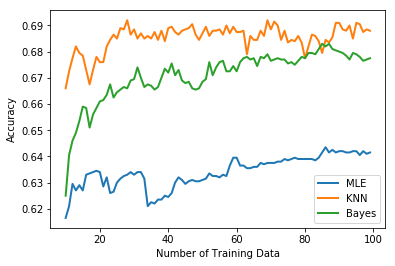
\includegraphics[scale=.5]{q5_fig/classifiers.png}	
		\caption{Prediction Accuracy against Size of Training Data}
	\end{figure}
\subsection*{(vi)}
	Demographic Parity is best achieved by MLE, having roughly $10\%$ difference in the probability of labelling $\hat{Y}=0$, 
	given different sensitive attributes.  
	\begin{figure}[H]
		\centering
		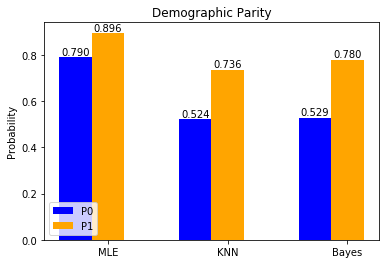
\includegraphics[scale=.5]{q5_fig/dp.png}	
		\caption{Demographic Parity Condition of Classifiers}
	\end{figure}
	Equalized Odds is best achieved by MLE, having $14.5\%$ difference in the probability of getting a true positive
	($\mathbb{P}_0[Y=1|\hat{Y}=1]-\mathbb{P}_1[Y=1|\hat{Y}=1]$),
	and $4.4\%$ difference in the probability of getting a true negative ($\mathbb{P}_0[Y=0|\hat{Y}=0]-\mathbb{P}_1[Y=0|\hat{Y}=0]$).
	\begin{figure}[H]
		\centering
		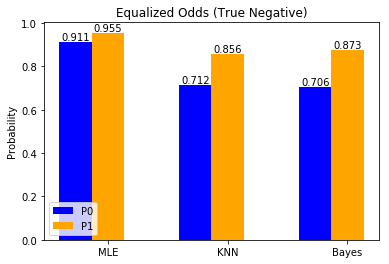
\includegraphics[scale=.5]{q5_fig/eo_neg.png}	
		\caption{Equalized True Negative Condition of Classifiers}
	\end{figure}
	\begin{figure}[H]
		\centering
		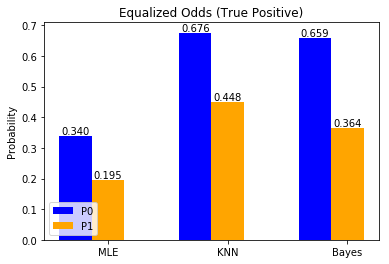
\includegraphics[scale=.5]{q5_fig/eo_pos.png}	
		\caption{Equalized True Positive Condition of Classifiers}
	\end{figure}
	KNN and Naive Bayes do similarity well for Predictive Parity. In particular, KNN has only $0.6\%$ difference in 
	negative predicative parity across the sensitive attribute.
	\begin{figure}[H]
		\centering
		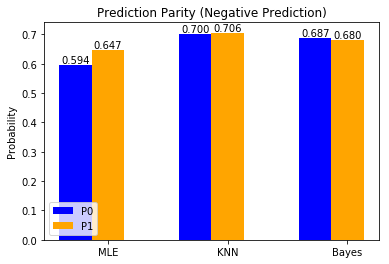
\includegraphics[scale=.5]{q5_fig/pp_neg.png}	
		\caption{Negative Predictive Parity Condition of Classifiers}
	\end{figure}
	\begin{figure}[H]
		\centering
		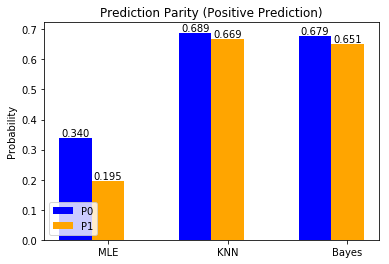
\includegraphics[scale=.5]{q5_fig/pp_pos.png}	
		\caption{Positive Predictive Parity Condition of Classifiers}
	\end{figure}
	In conclusion, the classification made by MLE favors Demographic Parity and Equalized Odds, while 
	KNN and Naive Bayes favor Predictive Parity.
\subsection*{(vii)}  
	Demographic Parity is applicable to job searches. Companies that use machine learning to select applicants need to make sure 
	that current bias in the labor market does not affect their future decision in hiring. 
	Research shows that male applicants with the same qualifications as female applicants get hired more often. 
	Demographic Parity could ensure that male and female applicants on average have the same probability of getting hired.
	The enforcement of Demographic Parity in short term benefits building up the reputation of the disadvantageous group 
	in the labor market in the long run.\\
	This definition, however, ignores any possible correlation between $Y$ and the sensitive attribute $A$. 
	In particular, it rules out perfect predictor $C=Y$ when base rates are different ($\mathbb{P}_0 [Y=1] \neq \mathbb{P}_1[Y=1]$).
	Moreover, if the employer hires the qualified male,
	and an unqualified female, demographic parity is still achieved. 


\subsection*{(viii)}  
	No, there is a tradeoff between bias and variance.


\section*{Problem 6}
\subsection*{(iii)}
	We consider three kinds of classifiers: naive-bayes, nearest neighbor (KNN), and decision tree. Here, we are working with word vectors with stop words and numbers removed, so as to improve runtime and reduce noise. Our data has been split so that 70% is allocated to training and 30% to testing.
	
	For KNN, we consider $L_1$, $L_2$, and $L_/infty$ norms for our distance metric. For k, we considered 1, 5, 10, 50, 100, 200, 500, and 1000.
	
		\begin{figure}[H]
		\centering
		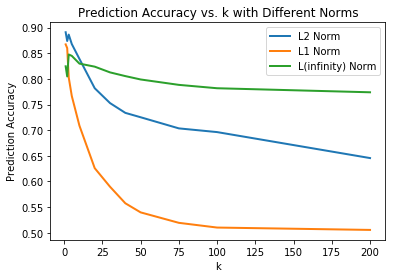
\includegraphics[scale=.5]{q6_fig/knn_k.png}	
		\caption{Prediction Accuracy vs. k with Different Norms}
	\end{figure}

	\begin{figure}[H]
		\centering
		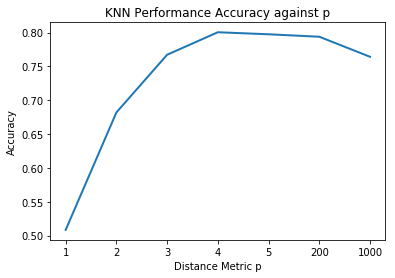
\includegraphics[scale=.5]{q6_fig/performance_vs_p.png}	
		\caption{Prediction Accuracy vs. k with Different Norms}
	\end{figure}
	
	We cohoe
	
	For the decision tree, we set aside 10\% of the training data as a validation set. To improve runtime and reduce noise, we consider only high variance features (features with the top 5\% variance).
	
	\begin{figure}[H]
		\centering
		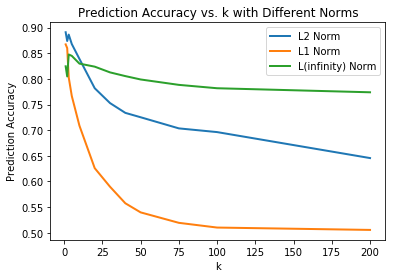
\includegraphics[scale=.5]{q6_fig/knn_k.png}	
		\caption{Prediction Accuracy vs. Decision Tree Depth}
	\end{figure}
	
		\begin{table}[H]
	\centering
	\caption{Performance of Classifiers}
	\begin{tabular}{lr}
		Classifier   & Accuracy \\
		\textbf{MLE}   & 0.6415    \\
		\textbf{KNN}   & 0.6895        \\
		\textbf{Bayes} & 0.9572
	\end{tabular}
	\end{table}
	
	
	




\end{document} 
